
\section{Derivatives}


\begin{frame}{Introduction}
    \begin{block}{Tangent Line}
        The \textbf{tangent line} to the curve $y=f(x)$ at the point $P(a, f(a))$ is the line through $P$ with slope
        $$
            m=\lim _{x \rightarrow a} \frac{f(x)-f(a)}{x-a}
        $$
        provided that this limit exists.
    \end{block}
    \begin{block}{Instantaneous rate of change}
        $$
            f^{\prime}(a)=\lim _{x \rightarrow a} \frac{f(x)-f(a)}{x-a}
        $$$$
            \text { instantaneous rate of change }=\lim _{\Delta x \rightarrow 0} \frac{\Delta y}{\Delta x}=\lim _{x_{2} \rightarrow x_{1}} \frac{f\left(x_{2}\right)-f\left(x_{1}\right)}{x_{2}-x_{1}}
        $$
    \end{block}
    Try to define velocity in this way.
\end{frame}



\begin{frame}{Introduction}
    $$
        \text{average velocity} = \frac{\text{displacement}}{\text{time}} = \frac{f(a+h)-f(a)}{h}
    $$
    $$v(a)=\lim _{h\rightarrow 0}\frac{f(a+h)-f(a)}{h}$$
\end{frame}



\begin{frame}{Definition}
    \begin{block}{Derivative}
        The \textbf{derivative of a function \boldmath{$f$} at a number \boldmath{$a$}}, denoted by $f'(a)$, is
        $$
            f^{\prime}(a)=\lim _{x \rightarrow a} \frac{f(x)-f(a)}{x-a}
        $$
        if this limit exists.
    \end{block}
    The slope of the tangent line of a function is the corresponding derivative.
\end{frame}



\begin{frame}{Definition}
    \begin{block}{Notations}
        Newton: $$
            \dot{y}
        $$
        Leibniz:
        $$
            \frac{d y}{d x}
        $$
        Lagrange:
        $$
            f^{\prime}(x)
        $$
        Jacobi: (Partial Derivatives)
        $$
            \frac{\partial f}{\partial x}
        $$
    \end{block}
\end{frame}



\begin{frame}{Differentiable}
    \begin{block}{Differentiable}
        A function $f$ is differentiable at $\boldsymbol{a}$ if $f^{\prime}(a)$ exists. It is differentiable on an open interval $(a, b)$ [or $(a, \infty)$ or $(-\infty, a)$ or $(-\infty, \infty)]$ if it is differentiable at every number in the interval.
    \end{block}
    \begin{block}{Differentiable and Continuity}
        If $f$ is differentiable at $a$, then $f$ is continuous at $a$.

        \textbf{NOTE} The converse of Theorem is false; that is, there are functions that are continuous but not differentiable. For instance, the function $f(x)=|x|$ is continuous at 0 because
        $$
            \lim _{x \rightarrow 0} f(x)=\lim _{x \rightarrow 0}|x|=0=f(0)
        $$
    \end{block}
\end{frame}



\begin{frame}{Differentiable}
    The function is not differentiable at these points:
    \bigskip
    \begin{figure}[htbp]
        \begin{center}
            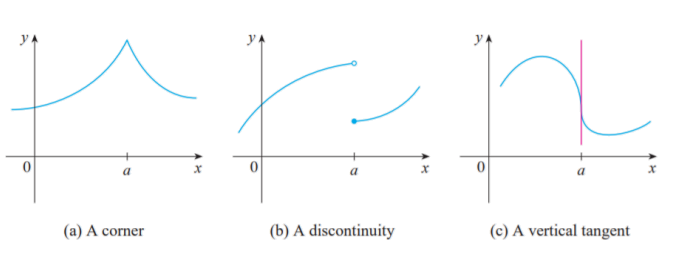
\includegraphics[width=1\textwidth]{res/4.png}
        \end{center}
    \end{figure}
\end{frame}



\begin{frame}{Higher derivatives}
    $$
        (f')' = f''\qquad \text{second derivative}
    $$$$
        (f'')' = f'''\qquad \text{third derivative}
    $$
    Example: still consider the position function
    \begin{center}
        position-velocity-acceleration-jerk-snap$\cdots$\\
        $$
            x-\frac{d y}{d t}-\frac{d^2 y}{d t^2}-\frac{d^3 y}{d t^3}-\frac{d^4 y}{d t^4}\cdots
        $$
    \end{center}
\end{frame}


\includepdf[pages=1]{Intro to Calculus.pdf}


\begin{frame}{Differential formulas}
    $$
        \frac{d}{d x}(C)=0
    $$$$
        \frac{d}{d x}(x^{n})=n x^{n-1}
    $$$$
        (c f)^{\prime}=c f^{\prime}
    $$$$
        (f+g)^{\prime}=f^{\prime}+g^{\prime}
    $$$$
        (f-g)^{\prime}=f^{\prime}-g^{\prime}
    $$$$
        (f g)^{\prime}=f g^{\prime}+g f^{\prime}
    $$$$
        (\frac{f}{g})^{\prime}=\frac{g f^{\prime}-f g^{\prime}}{g^{2}}
    $$
\end{frame}



\begin{frame}{Differential formulas}
    $$
        \begin{aligned}
             & \frac{d}{d x}(\sin x)=\cos x         \\
             & \frac{d}{d x}(\csc x)=-\csc x \cot x \\
             & \frac{d}{d x}(\cos x)=-\sin x        \\
             & \frac{d}{d x}(\sec x)=\sec x \tan x  \\
             & \frac{d}{d x}(\tan x)=\sec ^{2} x    \\
             & \frac{d}{d x}(\cot x)=-\csc ^{2} x
        \end{aligned}
    $$
\end{frame}



\begin{frame}{Differential formulas}
    $$
        \begin{aligned}
             & \frac{d}{d x}\left(\sin ^{-1} x\right)=\frac{1}{\sqrt{1-x^{2}}}    \\
             & \frac{d}{d x}\left(\csc ^{-1} x\right)=-\frac{1}{x \sqrt{x^{2}-1}} \\
             & \frac{d}{d x}\left(\cos ^{-1} x\right)=-\frac{1}{\sqrt{1-x^{2}}}   \\
             & \frac{d}{d x}\left(\sec ^{-1} x\right)=\frac{1}{x \sqrt{x^{2}-1}}  \\
             & \frac{d}{d x}\left(\tan ^{-1} x\right)=\frac{1}{1+x^{2}}           \\
             & \frac{d}{d x}\left(\cot ^{-1} x\right)=-\frac{1}{1+x^{2}}
        \end{aligned}
    $$
\end{frame}



\begin{frame}{Differential formulas}
    $$
        \begin{aligned}
             & \frac{d}{d x}\left(\log _{a} x\right)=\frac{1}{x \ln a} \\
             & \frac{d}{d x}(\ln x)=\frac{1}{x}                        \\
             & \frac{d}{d x} \ln |x|=\frac{1}{x}                       \\
        \end{aligned}
    $$
\end{frame}



\begin{frame}
    \frametitle{Exercise 1}
    \framesubtitle{Images of a Function and Its Derivative}
    Find an equation of the tangent line to the curve $y = 2x\sin{x}$ at the point ($\dfrac{\pi}{2}$, $\pi$).
\end{frame}



\begin{frame}
    \frametitle{Exercise 1}
    \framesubtitle{Images of a Function and Its Derivative}
    Find an equation of the tangent line to the curve $y = 2x\sin{x}$ at the point ($\dfrac{\pi}{2}$, $\pi$).
    
    \vspace*{1em}
    
    \textbf{Solution:}
    $y' = 2(sinx + xcosx)$
    
    $k = y'(\dfrac{\pi}{2}) = 2$
    
    $y - \pi = 2(x - \dfrac{\pi}{2})$
    
    $ y - 2x = 0$
\end{frame}

\begin{frame}{Exercise}
    \begin{block}{Composite Function}
        \begin{enumerate}
            \item If $g(x)=2 x+1$ and $h(x)=4 x^{2}+4 x+7$, find a function $f$ such that $f \circ g=h$. \\(Think about what operations you would have to perform on the formula for $g$ to end up with the formula for $h$.)\\
            \item If $f(x)=3 x+5$ and $h(x)=3 x^{2}+3 x+2$, find a function $g$ such that $f \circ g=h$.\\
        \end{enumerate}
    \end{block}
\end{frame}



\begin{frame}
    \frametitle{Exercise 2}
    \framesubtitle{Basic Derivation Formula}
    Differentiate:
    \begin{enumerate}
        \item $y = x^{3} + \dfrac{7}{x^{4}} - \dfrac{2}{x} + 12$
        \item $y = \sin{x}\cos{x}$
        \item $y = \sqrt{x}\sin{x}$
        \item $y = 3e^{x}\cos{x}$
        \item $y = \dfrac{x\sin{x}}{1 + x}$
        \item $y = \dfrac{1 - \sec{x}}{\tan{x}}$
        \item $y = x^{2}\ln{x}\cos{x}$
        \item $y = \ln{3} + \dfrac{e^{x}}{x^{2}}$
    \end{enumerate}
\end{frame}



\begin{frame}{Exercise 2}
    Solution:

    \begin{enumerate}
        \item $3x^2 - \dfrac{28}{x^5} + \dfrac{2}{x^2}$
        \item cos2x
        \item $\dfrac{1}{2}x^{-\frac{1}{2}}sinx + x^{\frac{1}{2}}cosx$
        \item $3e^x(-sinx + cosx)$
        \item $\dfrac{dy}{dx} = \dfrac{(xsinx)'(1+x)-xsinx}{(1+x)^2} = \dfrac{sinx + (1+x)xcosx}{(1+x)^2}$
        \item $y = \dfrac{cosx-1}{sinx}  \rightarrow \dfrac{dy}{dx} = \dfrac{1}{1+cosx}$
        \item $\dfrac{dy}{dx} = 2xlnxcosx + xcosx - x^2lnxsinx$
        \item $(-2x^{-3} + x^{-2})e^x$
    \end{enumerate}

\end{frame}

\colortheme{blue!50!black}


\begin{frame}
    \frametitle{Exercise 3}
    \framesubtitle{Basic Derivation Formula}
    Let $y = \log_{\varphi (x)}{f(x)}$\ ($\varphi (x) > 0$,\ $\varphi (x) \neq 1$,\ $f(x) > 0$). Suppose that both $\varphi (x)$ and $f(x)$ are differentiable. Calculate $\dfrac{dy}{dx}$.
\end{frame}



\begin{frame}{Exercise 3}
    Solution:

    $y = \dfrac{lnf(x)}{ln\varphi(x)}$

    $\dfrac{dy}{dx} = \dfrac{\frac{1}{f(x)}f'(x)ln\varphi(x) - \frac{1}{\varphi(x)}\varphi'(x)lnf(x)}{[ln\varphi(x)]^2}$

    $=\dfrac{f'(x)}{f(x)ln\varphi(x)} - \dfrac{\varphi'(x)lnf(x)}{\varphi(x)[ln\varphi(x)]^2}$

\end{frame}

\colortheme{green!30!black}



\begin{frame}{Chain rule}
    \begin{block}{Chain Rule}
        If $g$ is differentiable at $x$ and $f$ is differentiable at $g(x)$, then the composite function $F=f \circ g$ defined by $F(x)=f(g(x))$ is differentiable at $x$ and $F^{\prime}$ is given by the product
        $$
            F^{\prime}(x)=f^{\prime}(g(x)) \cdot g^{\prime}(x)
        $$
        In Leibniz notation, if $y=f(u)$ and $u=g(x)$ are both differentiable functions, then
        $$
            \frac{d y}{d x}=\frac{d y}{d u} \frac{d u}{d x}
        $$
    \end{block}
\end{frame}



\begin{frame}{Chain rule}
    \begin{block}{The Power Rule Combined with the Chain Rule }
        If $n$ is any real number and $u=g(x)$ is differentiable, then
        $$
            \frac{d}{d x}\left(u^{n}\right)=n u^{n-1} \frac{d u}{d x}
        $$
        Alternatively,
        $$
            \frac{d}{d x}[g(x)]^{n}=n[g(x)]^{n-1} \cdot g^{\prime}(x)
        $$
    \end{block}
\end{frame}


\begin{frame}
    \frametitle{Exercise 4}
    \framesubtitle{Chain Rule}
    Find the derivative of the function:
    \begin{enumerate}
        \item $y = (4x - x^{2})^{100}$
        \item $y = 5^{-\frac{1}{x}}$
        \item $y = e^{-2x}\cos{4x}$
        \item $y = (\dfrac{x^{2}+1}{x^{2}-1})^{3}$
        \item $y = \dfrac{\arcsin{x}}{\arccos{x}}$
        \item $y = [\sin{(e^{(\sin{x})^{2}})}]^{2}$
        \item $y = \arcsin{\sqrt{\dfrac{1 - x}{1 + x}}}$
        \item $y = n^{n^{x}} + x^{n^{n}} + n^{x^{n}}$\ ($n > 0$,\ $n \neq 1$)
    \end{enumerate}
\end{frame}



\begin{frame}{Exercise 4}
    \begin{enumerate}
        \item $200(2-x)(4x-x^2)^{99}$
        \item $ln5\cdot5^{-\frac{1}{x}}\cdot x^{-2}$
        \item $-2e^{-2x}(cos4x + 2sin4x)$
        \item $y' = 3(\dfrac{x^2+1}{x^2-1})^2(-\dfrac{2}{(x^2 - 1)^2})\cdot 2x = -\dfrac{12x(x^2+1)^2}{(x^2-1)^3}$
        \item $y' = \dfrac{(arcsinx)'arccosx - (arccosx)'arcsinx}{(arccosx)^2} = \dfrac{arccosx + arcsinx}{\sqrt{1-x^2}(arccosx)^2}$
        \item $y' = 2[sin(e^{(sinx)^2)}]\cdot cos(e^{(sinx)^2}) \cdot e^{(sinx)^2} \cdot 2sinxcosx = sin2x \cdot sin(2e^{(sinx)^2})\cdot e^{(sinx)^2}$
        \item $y' = (1-\dfrac{1-x}{1+x})^{-\frac{1}{2}}\cdot \dfrac{1}{2}(\dfrac{1-x}{1+x})^{-\dfrac{1}{2}}[-\dfrac{2}{(x+1)^2}] = -\dfrac{1}{\sqrt{2x(1-x)}\cdot (x+1)}$
        \item $y' = n^{n^x + x}(lnn)^2 + n^nx^{n^n -1} + n^{x^n + 1}x^{(n-1)}lnn$
    \end{enumerate}
\end{frame}



\begin{frame}
    \frametitle{Exercise 5}
    \framesubtitle{Higher Derivative}
    Find the second derivative of the following function:\\
    (\alert{Warning}: Don't forget to double check your first derivative!)
    \begin{enumerate}
        \item $y = \tan{x}$
        \item $y = \dfrac{1}{x^{3} + 1}$
        \item $y = x\cos{x}$
    \end{enumerate}
\end{frame}



\begin{frame}{Exercise 5}
    \begin{enumerate}
        \item $y' = sec^2x$

              $y'' = 2secx \cdot (tanx \cdot secx) = 2tanx \cdot sec^2x$
        \item $y' = -\dfrac{1}{(x^3 + 1)^2}\cdot 3x^2$

              $y'' = -3 \cdot \dfrac{2x(x^3+1)^2 - 2(x^3+1)3x^4}{(x^3 + 1)^4} = \dfrac{6x(2x^3 - 1)}{(x^3 + 1)^3}$
        \item $y' = cosx - xsinx$

              $y'' = -2sinx - xcosx$
    \end{enumerate}
\end{frame}



\begin{frame}
    \frametitle{Exercise 6}
    \framesubtitle{Higher Derivative}
    Answer the following three questions based on $\dfrac{dy}{dx} = y'$:
    \begin{enumerate}
        \item Express $\dfrac{dx}{dy}$ with $y'$
        \item Express $\dfrac{d^{2}x}{dy^{2}}$ with $y'$ and $y''$
        \item Express $\dfrac{d^{3}x}{dy^{3}}$ with $y'$ ,$y''$ and $y'''$
    \end{enumerate}
\end{frame}



\begin{frame}{Exercise 6}
    Solution:
    \begin{enumerate}
        \item $\dfrac{dx}{dy} = \dfrac{1}{dy/dx} = \dfrac{1}{y'}$
        \item $\dfrac{d^2x}{dy^2} = \dfrac{d}{dy}\cdot \dfrac{dx}{dy} = \dfrac{d}{dx}\dfrac{1}{y'}\dfrac{dx}{dy} = -\dfrac{y''}{(y')^3}$
        \item $\dfrac{d^3x}{dy^3} = \dfrac{d}{dy}\dfrac{d^2x}{dy^2} = \dfrac{d}{dx}\dfrac{d^2x}{dy^2}\dfrac{dx}{dy} = - \dfrac{y'''(y')^3 - 3(y')^2(y'')^2}{(y')^6}\cdot \dfrac{1}{y'} = \dfrac{3(y'')^2 - y' (y''')^2}{(y')^5}$
    \end{enumerate}

\end{frame}



\begin{frame}{Implicit Differentiation}
    \begin{block}{Find $y^{\prime}$ if $\sin (x+y)=y^{2} \cos x$}
        Differentiating implicitly with respect to $x$ and remembering that $y$ is a function of $x$, we get
        $$
            \cos (x+y) \cdot\left(1+y^{\prime}\right)=y^{2}(-\sin x)+(\cos x)\left(2 y y^{\prime}\right)
        $$
        (Note that we have used the Chain Rule on the left side and the Product Rule and Chain Rule on the right side.) If we collect the terms that involve $y^{\prime}$, we get
        $$
            \cos (x+y)+y^{2} \sin x=(2 y \cos x) y^{\prime}-\cos (x+y) \cdot y^{\prime}
        $$
        So
        $$
            y^{\prime}=\frac{y^{2} \sin x+\cos (x+y)}{2 y \cos x-\cos (x+y)}
        $$
    \end{block}
\end{frame}


\begin{frame}
    \frametitle{Exercise 7}
    \framesubtitle{Implicit Differentiation}
    Calculate the derivative of the following implicit function:
    \begin{enumerate}
        \item $y^{2} - 2xy + 9 = 0$
        \item $xy = e^{xy}$
    \end{enumerate}
\end{frame}


\begin{frame}{Solution}
    \begin{enumerate}
        \item $2yy'-2y-2xy'=0$,$y'=\dfrac{y}{y-x}$
        \item The derivative does not exist!
    \end{enumerate}
\end{frame}


\begin{frame}
    \frametitle{Exercise 8}
    \framesubtitle{Implicit Differentiation}
    Use \alert{logarithmatic differentiation} to calculate the derivative of the following implicit function:
    \begin{enumerate}
        \item $y = (\dfrac{x}{x + 1})^{x}$
        \item $y = \sqrt[5]{\dfrac{x - 5}{\sqrt[5]{x^{2} + 2}}}$
    \end{enumerate}
\end{frame}



\begin{frame}{Exercise 8}
    Solution:
    \begin{enumerate}
        \item $lny = x[lnx - ln(x+1)]$

              $\dfrac{1}{y}y' = [lnx - ln(x+1)] + x[\dfrac{1}{x} - \dfrac{1}{x+1}]$

              $y' = (\dfrac{x}{x+1})^x [ln|\dfrac{x}{x+1}| + \dfrac{1}{x+1}]$
        \item $lny = \dfrac{1}{5}ln|x-5| - \dfrac{1}{25}ln(x^2 + 2)$

              $y'\dfrac{1}{y} = \dfrac{1}{5(x-5)} - \dfrac{2x}{25(x^2+2)}$

              $y' = y[\dfrac{1}{5(x-5)} - \dfrac{2x}{25(x^2+2)}]$
    \end{enumerate}
\end{frame}




\begin{frame}
    \frametitle{Exercise 9}
    \framesubtitle{Implicit Differentiation}
    The \textit{Bessel function} of order $0, y=J(x)$, satisfies the differential equation $x y^{\prime \prime}+y^{\prime}+x y=0$ for all values of $x$ and its value at 0 is $J(0)=1$.\\
    (a) Find $J^{\prime}(0)$.\\
    (b) Use implicit differentiation to find $J^{\prime \prime}(0)$.
\end{frame}



\begin{frame}{Exercise 9}
    Solution:
    \begin{enumerate}
        \item Take x=0, 0 + J'(0) + 0 = 0 $\rightarrow$ J'(0) = 0
        \item xy''' + 2y'' + y + xy' = 0

              At x = 0, 2y'' + 1 = 0, y'' = $-\dfrac{1}{2}$
    \end{enumerate}

\end{frame}


\begin{frame}
    \frametitle{More Exercises}
    \begin{block}{10.}
        Find the derivative of the function $\displaystyle f(x)=(x\sin^2(x))^{\frac{1}{3}}$.
    \end{block}

    \begin{block}{11.}
        The equation of the tangent to $f(x)$ at $x=1$ is $y=-2(x-3)$, and knowing that $g(x) = f^{-1}+3$, find the equation of the tangent to $g(x)$ at $x=3$.
    \end{block}

    \begin{block}{12.}
        Find the slope of the tangent to the curve $xy = \arctan(3y)$ when $y = \dfrac{1}{3}$.
    \end{block}

\end{frame}


\begin{frame}{Linear approximation}
    \begin{block}{Definition}

        $$
            f(x) \approx f(a)+f^{\prime}(a)(x-a)
        $$
        is called the \textbf{linear approximation} or \textbf{tangent line approximation} of $f$ at $a$. The linear function whose graph is this tangent line, that is,\\

        $$
            L(x)=f(a)+f^{\prime}(a)(x-a)
        $$
        is called the linearization of $f$ at $a$.
    \end{block}
\end{frame}


\begin{frame}{Exercise 10}
    \begin{block}{}
        Use linear approximation to estimate $2.0006^{1.9998}$
    \end{block}
\end{frame}



\begin{frame}{Exercise 10}
    Solution:

    \linespread{2}

    $f(x) = 2^{x+2}$

    $f'(x) = 2^{x+2}ln2$

    $2^{1.9998} = f(0) + f'(0) \times (-0.0002) =  2^2 + 4ln2 \times (-0.0002) = 3.9994$

    $g(x) = (2+x)^{1.9998}$

    $g'(x) = 1.9998(2+x)^{0.9998}$

    $2.0006^{1.9998} = g(0) + g'(0)\times 0.0006 = 2^{1.9998} + 1.9998\times 2^{0.9998}\times 0.0006 = 4.0018$

\end{frame}



% \begin{frame}{Equivalent Infinitesimal}
%     \textbf{Tip:} You're highly recommended to remember this part!
%     $$
%         \begin{aligned}
%              & \textbf{When } x \rightarrow 0          \\
%              & a^{x}-1 \sim x \ln a                    \\
%              & \arcsin (a) x \sim \sin (a) x \sim(a) x \\
%              & \arctan (a) x \sim \tan (a) x \sim(a) x \\
%              & \ln (1+x) \sim x                        \\
%              & \sqrt{1+x}-\sqrt{1-x} \sim x            \\
%              & (1+a x)^{b}-1 \sim a b x                \\
%              & \sqrt[b]{1+a x}-1 \sim \frac{a}{b} x    \\
%              & 1-\cos x \sim \frac{x^{2}}{2}           \\
%              & x-\ln (1+x) \sim \frac{x^{2}}{2}        \\
%         \end{aligned}
%     $$
% \end{frame}




% \begin{frame}{Equivalent Infinitesimal}
%     $$
%         \begin{aligned}
%              & \textbf{When } x \rightarrow 0     \\
%              & \tan x-\sin x \sim \frac{x^{3}}{2} \\
%              & \tan x-x \sim \frac{x^{3}}{3}      \\
%              & x-\arctan x \sim \frac{x^{3}}{3}   \\
%              & x-\sin x \sim \frac{x^{3}}{6}      \\
%              & \arcsin x-x \sim \frac{x^{3}}{6}   \\
%         \end{aligned}
%     $$
% \end{frame}



% \colortheme{green!30!black}


\begin{frame}{Maximum and minimum}
    \begin{block}{Absolute Maximum and Absolute Minimum}
        Let $c$ be a number in the domain $D$ of a function $f$. Then $f(c)$ is the

        - \textbf{absolute maximum} value of $f$ on $D$ if $f(c) \geqslant f(x)$ for all $x$ in $D$.

        - \textbf{absolute minimum} value of $f$ on $D$ if $f(c) \leqslant f(x)$ for all $x$ in $D$.
    \end{block}
    \begin{block}{Local Maximum and Local Minimum}
        The number $f(c)$ is a

        - \textbf{local maximum} value of $f$ if $f(c) \geqslant f(x)$ when $x$ is near $c$.

        - \textbf{local minimum} value of $f$ if $f(c) \leqslant f(x)$ when $x$ is near $c$.
    \end{block}
    \begin{block}{Critical number}
        A \textbf{critical number} of a function $f$ is a number $c$ in the domain such that either $f^\prime (c)=0$ or $f^\prime (c)$ does not exist, or the end points of a region if it is bounded.
    \end{block}
    local maximum/minimum $\rightarrow$ critical number
\end{frame}



\begin{frame}{Related Theorems}
    \begin{block}{The Extreme Value Theorem}
        If $f$ is continuous on a closed interval $[a, b]$, then $f$ attains an absolute maximum value $f(c)$ and an absolute minimum value $f(d)$ at some numbers $c$ and $d$ in $[a, b]$.
    \end{block}
    \begin{block}{Fermat's Theorem}
        If $f$ has a local maximum or minimum at $c$, and if $f^{\prime}(c)$ exists, then $f^{\prime}(c)=0$.
    \end{block}
    \begin{block}{Rolle's Theorem}
        Let $f$ be a function that satisfies the following three hypotheses:

        1. $f$ is continuous on the closed interval $[a, b]$.

        2. $f$ is differentiable on the open interval $(a, b)$.

        3. $f(a)=f(b)$

        Then there is a number $c$ in $(a, b)$ such that $f^{\prime}(c)=0$.
    \end{block}
\end{frame}


\begin{frame}{Related Theorems}
    \begin{block}{Lagrange Mean Value Theorem }
        Let $f$ be a function that satisfies the following hypotheses:

        1. $f$ is continuous on the closed interval $[a, b]$.

        2. $f$ is differentiable on the open interval $(a, b)$.

        Then there is a number $c$ in $(a, b)$ such that
        $$
            f^{\prime}(c)=\frac{f(b)-f(a)}{b-a}
        $$
        or, equivalently,
        $f(b)-f(a)=f^{\prime}(c)(b-a)$
    \end{block}
\end{frame}


\begin{frame}{Related Theorems}
    \begin{block}{Cauchy Mean Value Theorem (Extended Mean Value Theorem) }
        Let $f,g$ be two functions that satisfy the following hypotheses:

        1. $f,g$ is continuous on the closed interval $[a, b]$.

        2. $f,g$ is differentiable on the open interval $(a, b)$.

        3.$x \in(a, b), g^{\prime}(x) \neq 0$

        Then there is a number $c$ in $(a, b)$ such that
        $$
            \frac{f(b)-f(a)}{g(b)-g(a)}=\frac{f^{\prime}(c)}{g^{\prime}(c)}
        $$
        or, equivalently,
        $(f(b)-f(a)) g^{\prime}(c)=(g(b)-g(a)) f^{\prime}(c)$
    \end{block}
\end{frame}



\begin{frame}
    \frametitle{Exercise 12}
    \framesubtitle{The Mean Value Theorem}
    Verify that the function satisfies the hypotheses of the Mean Value Theorem on the given interval. Then find all numbers $c$ that satisfy the conclusion of the Mean Value Theorem.
    \begin{enumerate}
        \item $f(x)=x^{3}-3 x+2, \quad[-2,2]$
        \item $f(x)=\ln x, \quad[1,4]$
    \end{enumerate}
\end{frame}



\begin{frame}{Exercise 12}
    Solutions:
    \begin{enumerate}
        \item f(-2) = 0, f(2) = 4

              $k = \dfrac{f(2) - f(-2)}{4} = 1$

              $f'(x) = 3x^2 - 3, 3c^2 - 3 = 1$

              $c = \dfrac{2\sqrt{3}}{3}$
        \item
              $k = \dfrac{f(4) - f(1)}{3} = \dfrac{2ln2}{3}$

              $f'(x) = \dfrac{1}{x}$

              $d = \dfrac{3}{2ln2}$

    \end{enumerate}
\end{frame}





\begin{frame}{Relationship between $f^\prime$ and $f$}
    \begin{block}{Increasing/Decreasing Test}
        If $f^\prime(x)>0$ on an interval, then $f$ is increasing on that interval.\\
        If $f^\prime(x)<0$ on an interval, then $f$ is decreasing on that interval.\\
    \end{block}
    \begin{block}{The First Derivative Test}
        Suppose that $c$ is a critical number of a continuous function $f$.\\
        If $f^\prime$ changes from positive to negative at $c$, $f$ has a local maximum at $c$.\\
        If $f^\prime$ changes from negative to positive at $c$, $f$ has a local minimum at $c$.\\
        If $f^\prime$ does not change sign at $c$, $f$ has no local maximum or minimum at $c$.
    \end{block}
\end{frame}



\begin{frame}{Relationship between $f^{\prime\prime}$ and $f$}
    \begin{block}{Concave upward/downward}
        If the graph of $f$ lies above all of its tangents on an interval $I$, then it is called \textbf{concave upward} on $I$. If the graph of $f$ lies below all of its tangents on an interval $I$, then it is called \textbf{concave downward} on $I$.
    \end{block}
    \begin{block}{Concavity Test}
        If $f^{\prime\prime}(x)>0$ for all $x$ in $I$, then the graph of $I$ is concave upward on $I$.\\
        If $f^{\prime\prime}(x)<0$ for all $x$ in $I$, then the graph of $I$ is concave downward on $I$.
    \end{block}
\end{frame}



\begin{frame}{Relationship between $f^{\prime\prime}$ and $f$}
    \begin{block}{Inflection point}
        A point $P$ on a curve $y=f(x)$ is called an \textbf{inflection point} if $f$ is continuous there and the curve changes from concave upward to concave downward or from concave downward to concave upward at $P$.
    \end{block}
    \begin{block}{The Second Derivative Test}
        Suppose $f^{\prime\prime}$ is continuous near $c$.\\
        If $f^\prime(c)=0$ and $f^{\prime\prime}(c)>0$, then $f$ has a local minimum at $c$.\\
        If $f^\prime(c)=0$ and $f^{\prime\prime}(c)<0$, then $f$ has a local maximum at $c$.
    \end{block}
\end{frame}



\begin{frame}{References}

    [1] Huang, Yucheng. VV156\_RC2.pdf. 2021.\\
    \bigskip
    [2] Huang, Yucheng. VV156\_RC3.pdf. 2021.\\
    \bigskip
    [3] Cai, Runze. Chapter02.pdf. 2021.\\
    \bigskip
    [4] Cai, Runze. Chapter03.pdf. 2021.\\
    \bigskip
    [5] Department of mathematics, Tongji University. Advanced Mathematics (7th Edition). 2014.\\
    \bigskip
    [6] James Stewart. Calculus (7th Edition). 2014.\\
    \bigskip
    [7] Department of mathematics, Tongji University. Learning Guidance of Advanced Mathematics (7th Edition). 2014.\\
    \bigskip
    [8]Huang, Jiahe, Zhou Yishen. VV156 RC3. 2022\\
\end{frame}
